%!TEX root = icwsm2017_poster.tex

%%%%%%%%%%%%%%%%%%%%%%%%%%%%%%%%%%%%%%%%%%%%%%%%%%%%%%%%%%%%%%%%%%%%%%%%%%%
%\begin{figure}[h!]
%\centering
%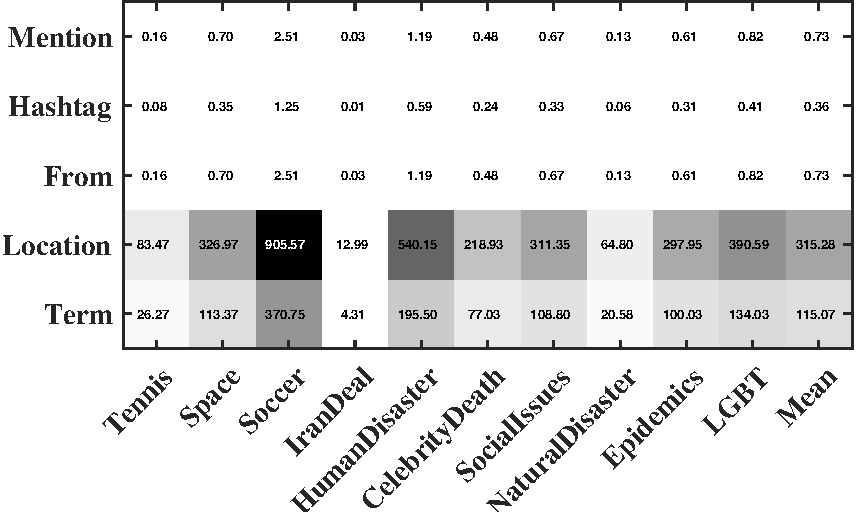
\includegraphics[width=0.5\textwidth]{images/medianMI.pdf}
%\vspace{-3mm}
%\caption{Median MI for different features vs. Topics, last two column show mean value and stderr across all topics}
%\label{fig:medianMI}
%\end{figure}
\begin{figure}[t!]
\centering
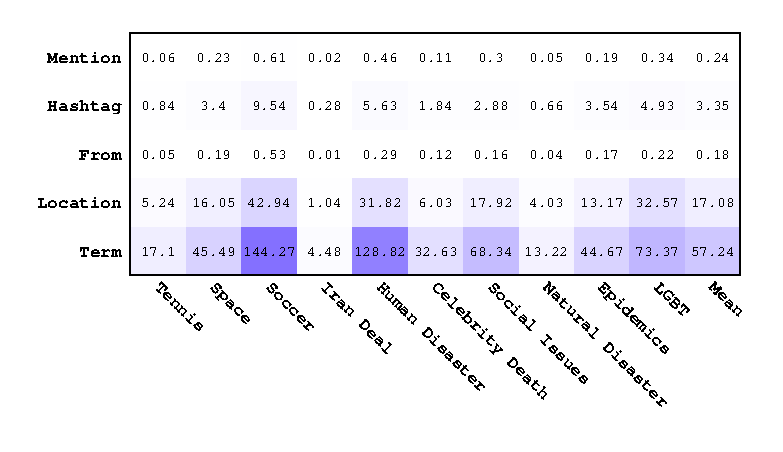
\includegraphics[height=48mm]{images/avgMI_gray2.eps}
%\vspace{-3mm}
\caption{Matrix of mean Mutual Information values (divided by $1E+10$ for different feature types vs. topics.  The last column is the average of mean values across all topics.)}
\label{fig:avgMI}
\end{figure}
%%%%%%%%%%%%%%%%%%%%%%%%%%%%%%%%%%%%%%%%%%%%%%%%%%%%%%%%%%%%%%%%%%%%%%%%%%%

%%%%%%%%%%%%%%%%%%%%%%%%%%%%%%%%%%%%%%%%%%%%%%%%%%%%%%%%%%%%%%%%%%%%%%%%%%%%
%\begin{figure*}[tp!]
%\centering
%\begin{tabular}{ccccc}
%%\fbox{\rule{10cm}{3.85cm}}
%\subfloat[Fig:][]{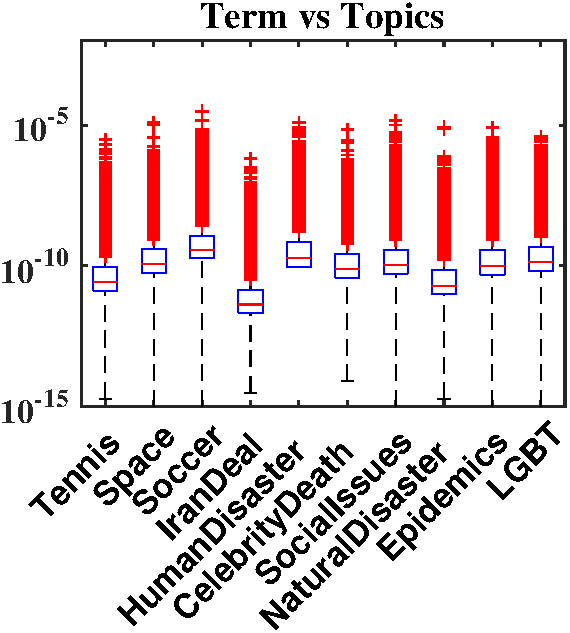
\includegraphics[width=34mm, height=35mm]{images/avgMIBoxPlots/TermVsTopics.pdf}}
%\subfloat[Fig:][]{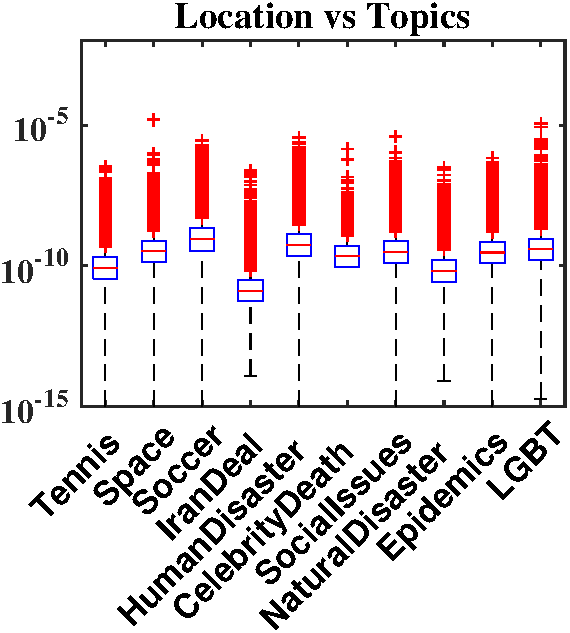
\includegraphics[width=34mm, height=35mm]{images/avgMIBoxPlots/LocationVsTopics.pdf}}
%\subfloat[Fig:][]{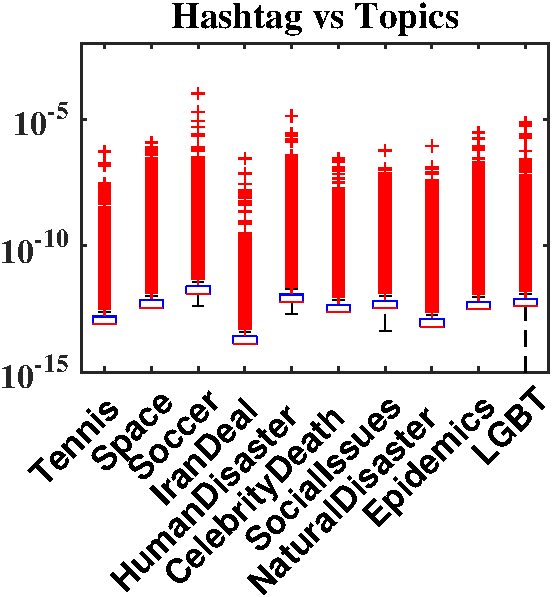
\includegraphics[width=34mm, height=35mm]{images/avgMIBoxPlots/HashtagVsTopics.pdf}}
%\subfloat[Fig:][]{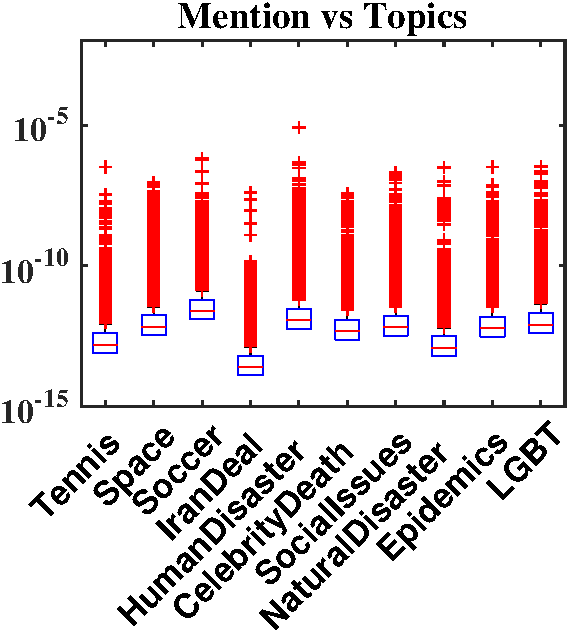
\includegraphics[width=34mm, height=35mm]{images/avgMIBoxPlots/MentionVsTopics.pdf}}
%\subfloat[Fig:][]{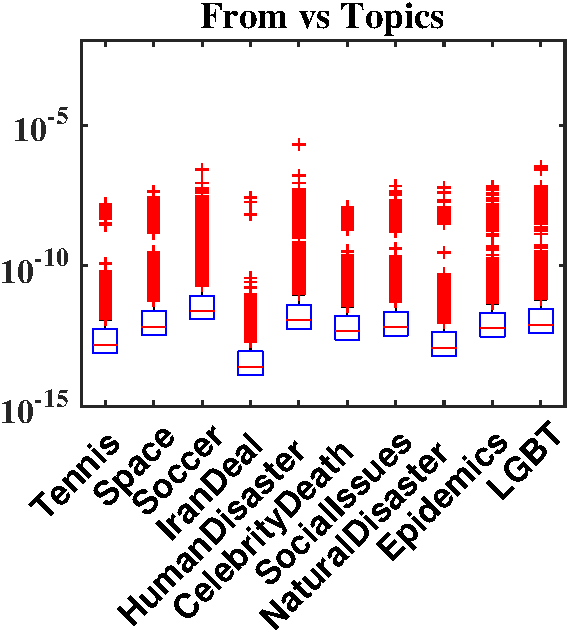
\includegraphics[width=34mm, height=35mm]{images/avgMIBoxPlots/FromVsTopics.pdf}} \\
%\end{tabular}
%%\vspace{-2mm}
%\caption {Box plots of Mutual Information values (y-axis) per feature type across topics (x-axis labels).}
%\label{fig:avgMIBP}
%%\vspace{2mm} commented due to AAAI Formating
%\end{figure*}
%%%%%%%%%%%%%%%%%%%%%%%%%%%%%%%%%%%%%%%%%%%%%%%%%%%%%%%%%%%%%%%%%%%%%%%%%%%%

%%%%%%%%%%%%%%%%%%%%%%%%%%%%%%%%%%%%%%%%%%%%%%%%%%%%%%%%%%%%%%%%%%%%%%%%%%%
\COMMENT
\begin{figure*}[tp!]
\centering
\begin{tabular}{ccccc}
\begin{tabular}{ccccc} % height=35mm -- always scale graphics proportionally by just specifying one dim. -SPS
\subfloat[Fig:][]{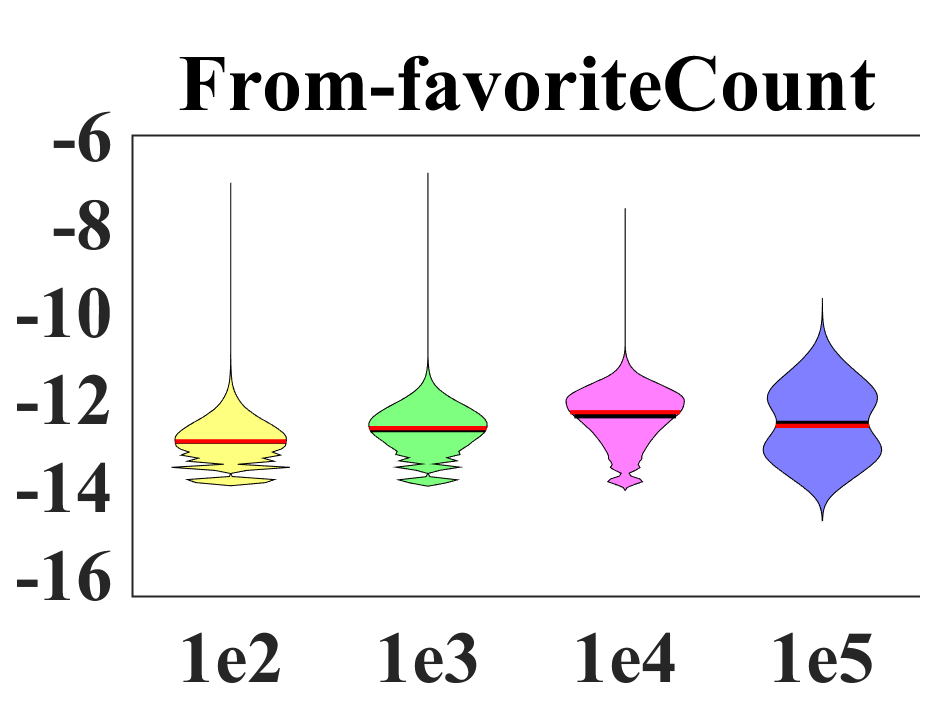
\includegraphics[width=34mm]{images/ViolinPlots/From-favoriteCount.eps}}
\subfloat[Fig:][]{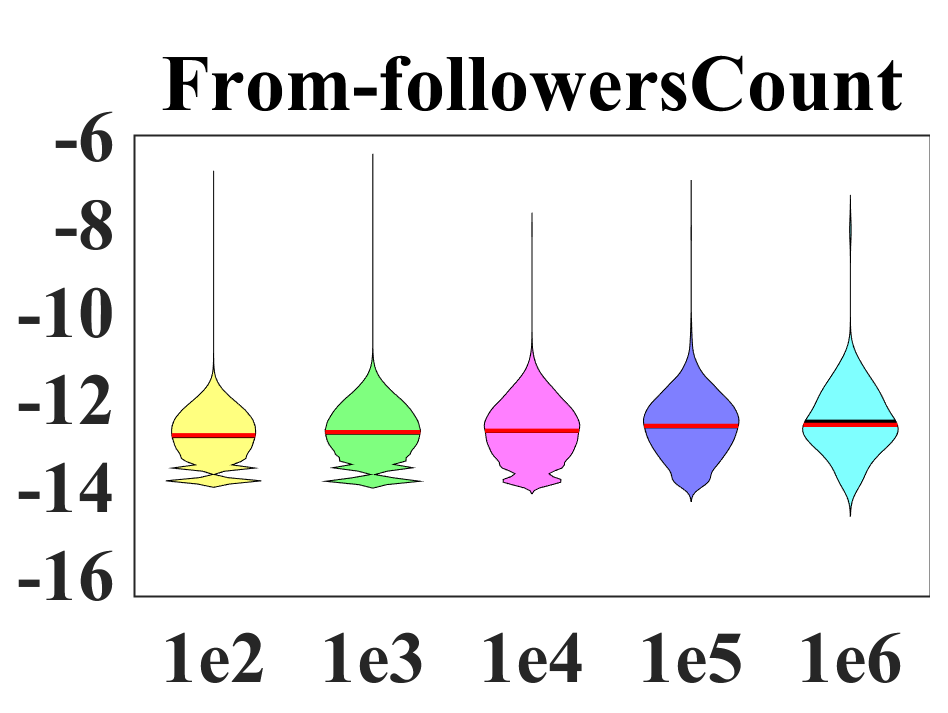
\includegraphics[width=34mm]{images/ViolinPlots/From-followersCount.eps}}
\subfloat[Fig:][]{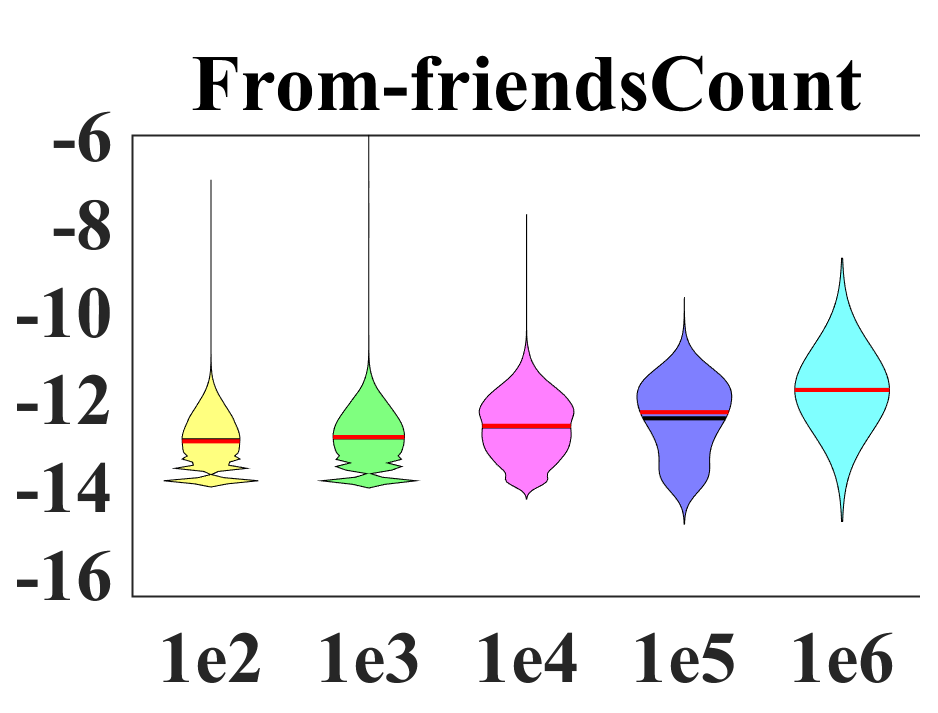
\includegraphics[width=34mm]{images/ViolinPlots/From-friendsCount.eps}}
\subfloat[Fig:][]{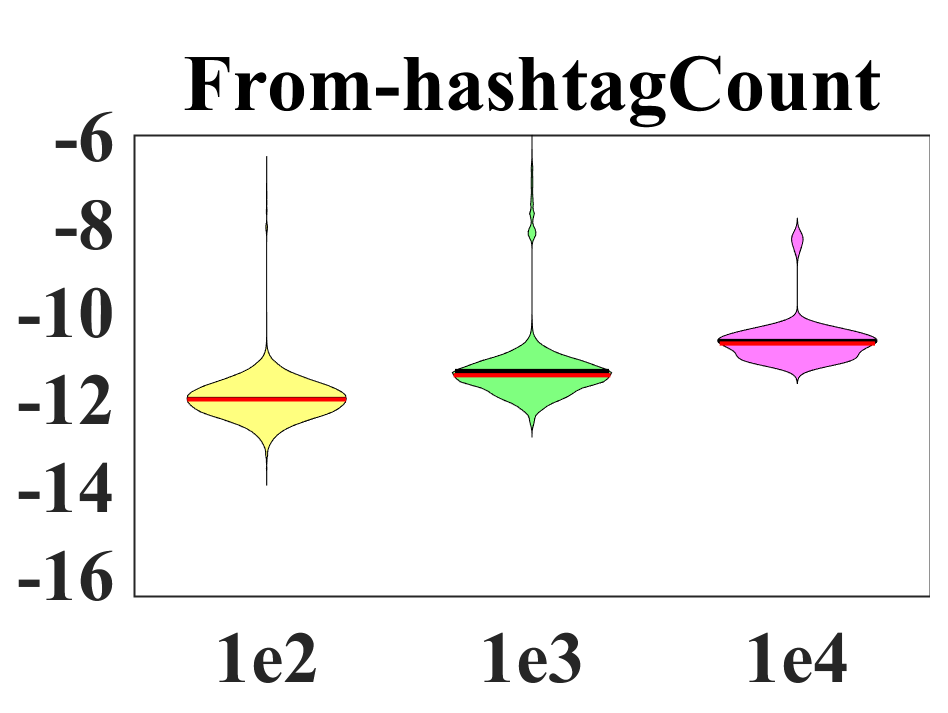
\includegraphics[width=34mm]{images/ViolinPlots/From-hashtagCount.eps}}
\subfloat[Fig:][]{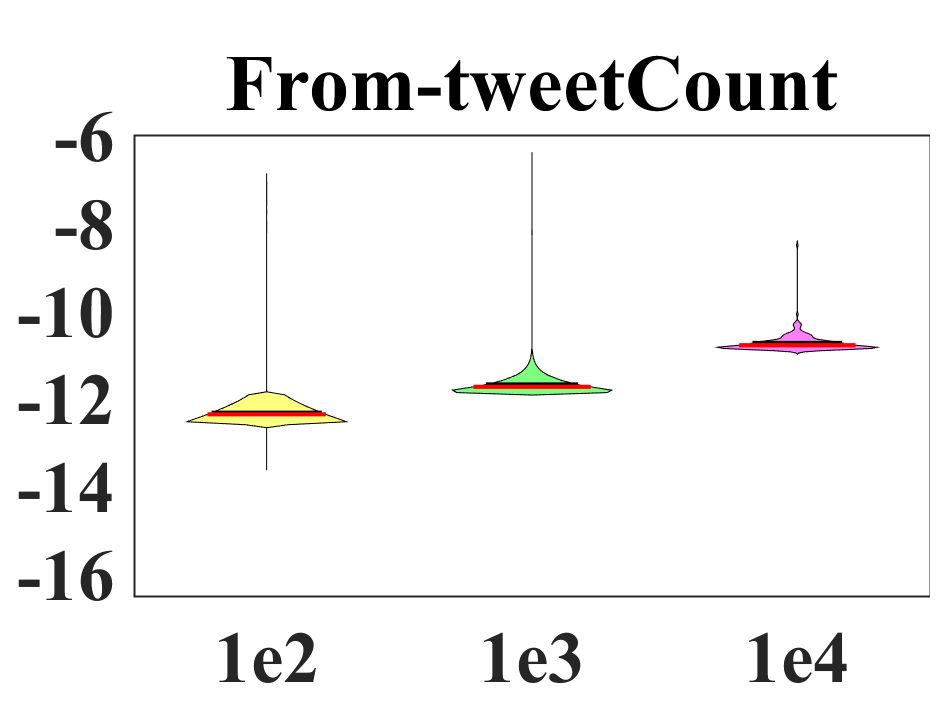
\includegraphics[width=34mm]{images/ViolinPlots/From-tweetCount.eps}} \\
%\vspace{-10mm}
\subfloat[Fig:][]{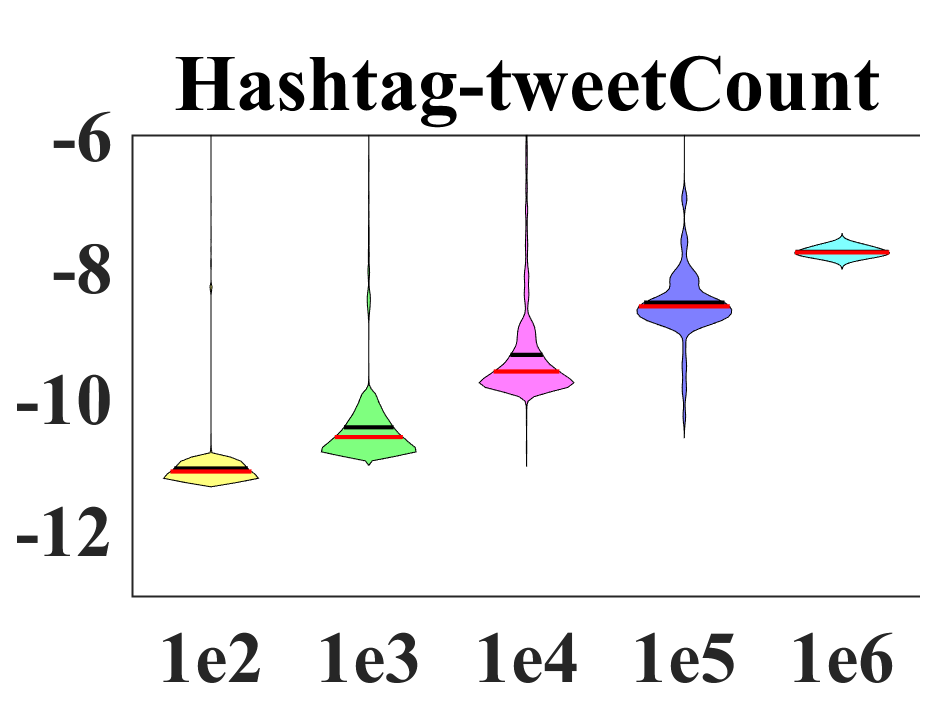
\includegraphics[width=34mm]{images/ViolinPlots/Hashtag-tweetCount.eps}}
\subfloat[Fig:][]{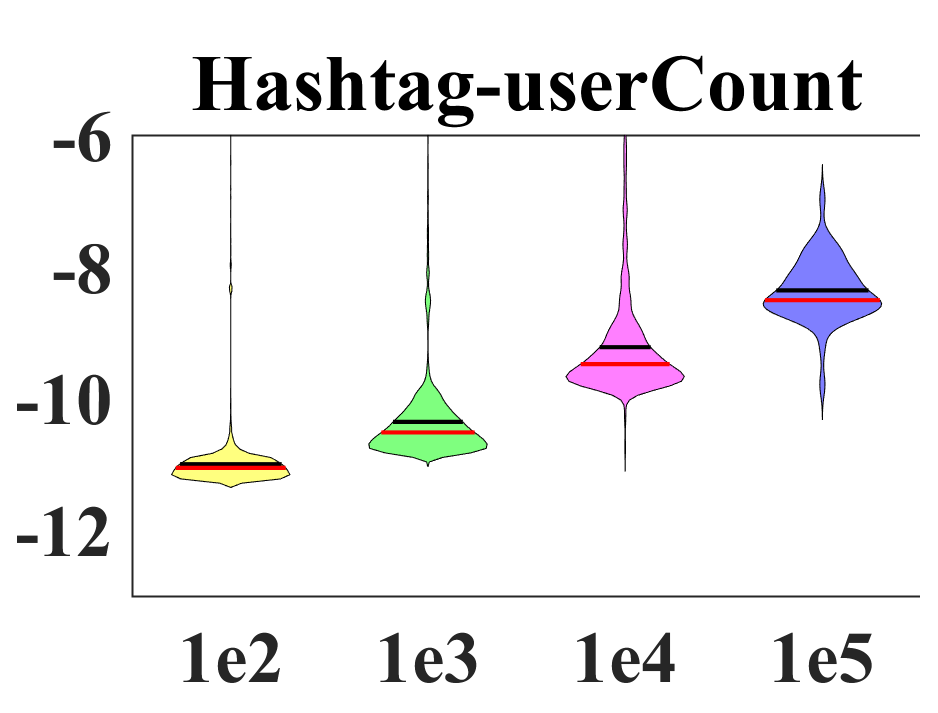
\includegraphics[width=34mm]{images/ViolinPlots/Hashtag-userCount.eps}}
\subfloat[Fig:][]{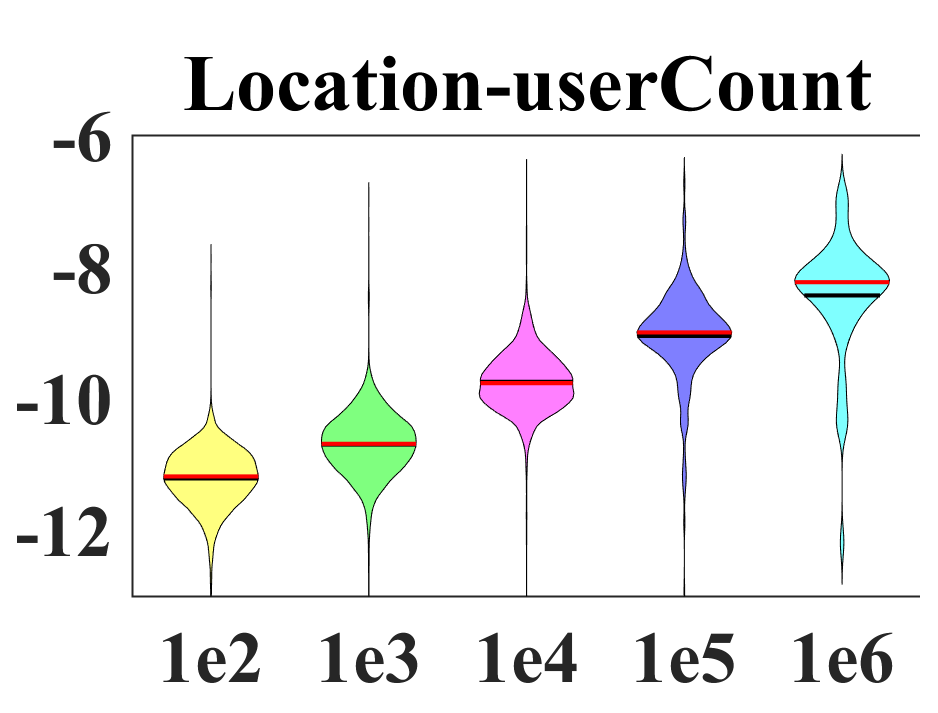
\includegraphics[width=34mm]{images/ViolinPlots/Location-userCount.eps}}
\subfloat[Fig:][]{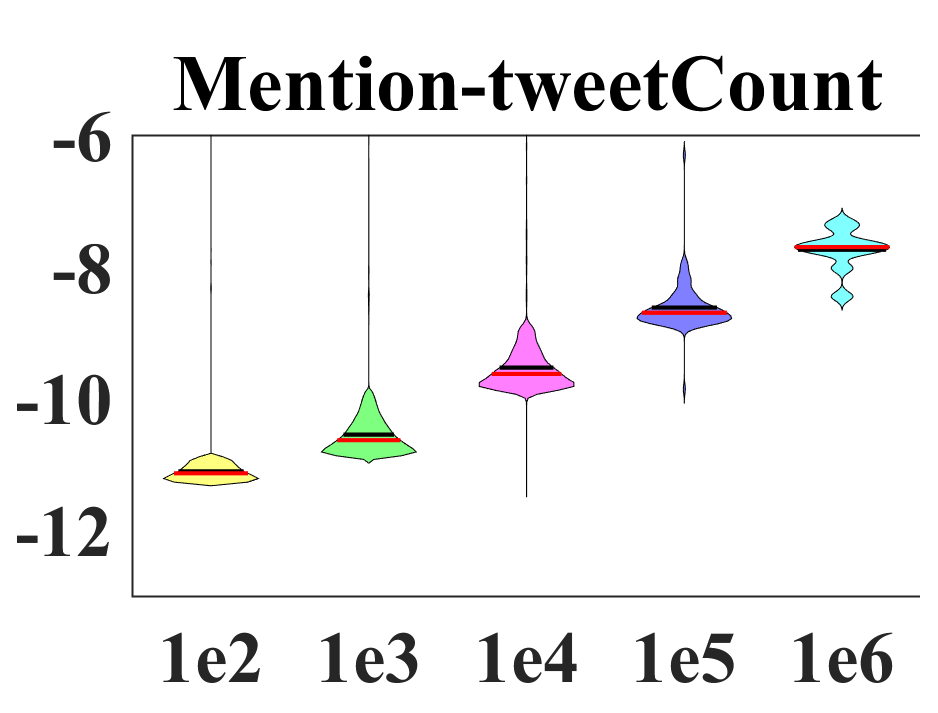
\includegraphics[width=34mm]{images/ViolinPlots/Mention-tweetCount.eps}}
\subfloat[Fig:][]{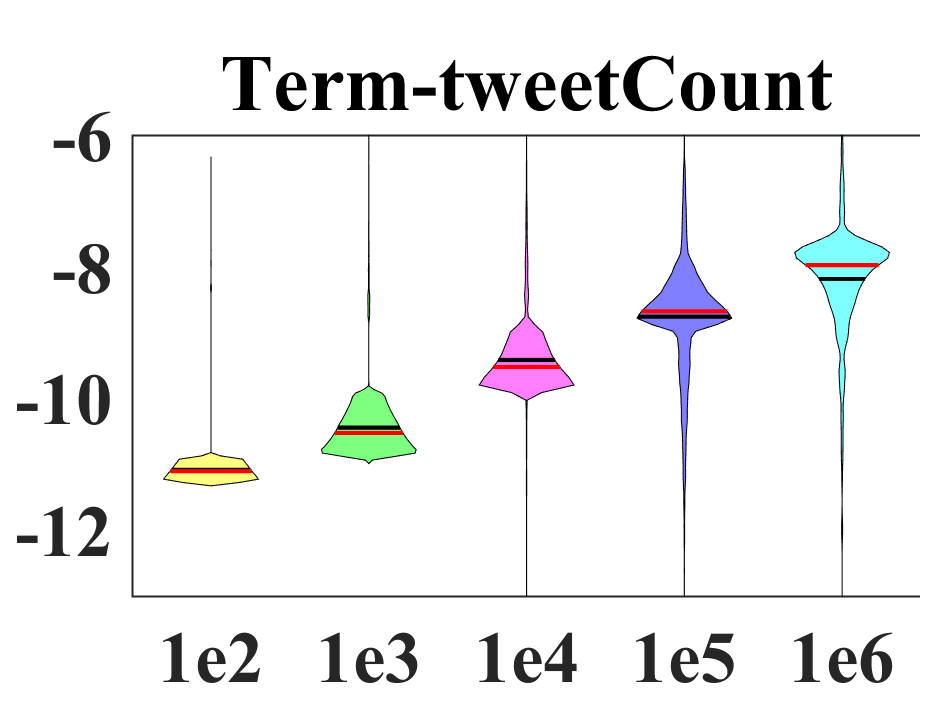
\includegraphics[width=34mm]{images/ViolinPlots/Term-tweetCount.eps}} \\
\end{tabular}
\end{tabular}
%\vspace{-2mm}
\caption {Violin plots for the distribution of Mutual Information values (y-axis) of different features as a function of their attribute values (binned on x-axis).  Plots (a-e) respectively show attributes \{favoriteCount, followerCount, friendCount, hashtagCount, tweetCount\} for \textit{From} feature. Plots (f-j) respectively show attributes tweetCount and userCount for \textit{Hashtag}, userCount for \textit{Location} feature, tweetCount for \textit{Mention} and \textit{Term} features.}
\label{fig:violinplots}
%\vspace{2mm} commented due to AAAI Formating
\end{figure*}
\ENDCOMMENT
%%%%%%%%%%%%%%%%%%%%%%%%%%%%%%%%%%%%%%%%%%%%%%%%%%%%%%%%%%%%%%%%%%%%%%%%%%%

%%%%%%%%%%%%%%%%%%%%%%%%%%%%%%%%%%%%%%%%%%%%%%%%%%%%%%%%%%%%%%%%%%%%%%%%%%%
\COMMENT
\begin{figure*}[tp!]
\centering
\begin{tabular}{cccc} % height=35mm -- always scale graphics proportionally by just specifying one dim. -SPS
\subfloat[Fig:][]{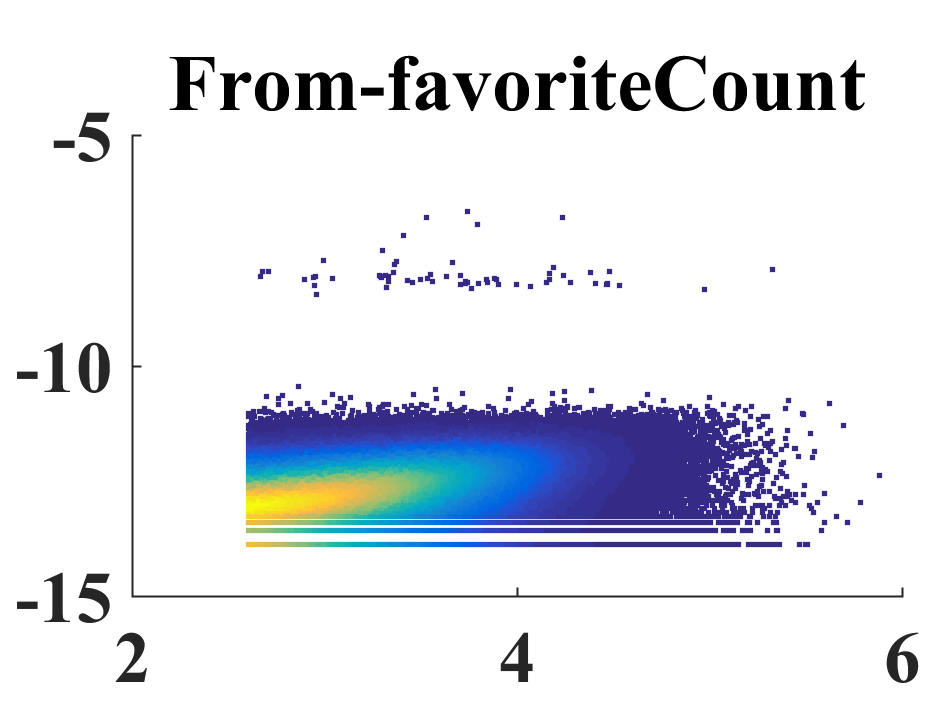
\includegraphics[width=40mm]{images/DensityPlots_IranDeal/dscatterPlot_From-favoriteCount.eps}} \quad
\subfloat[Fig:][]{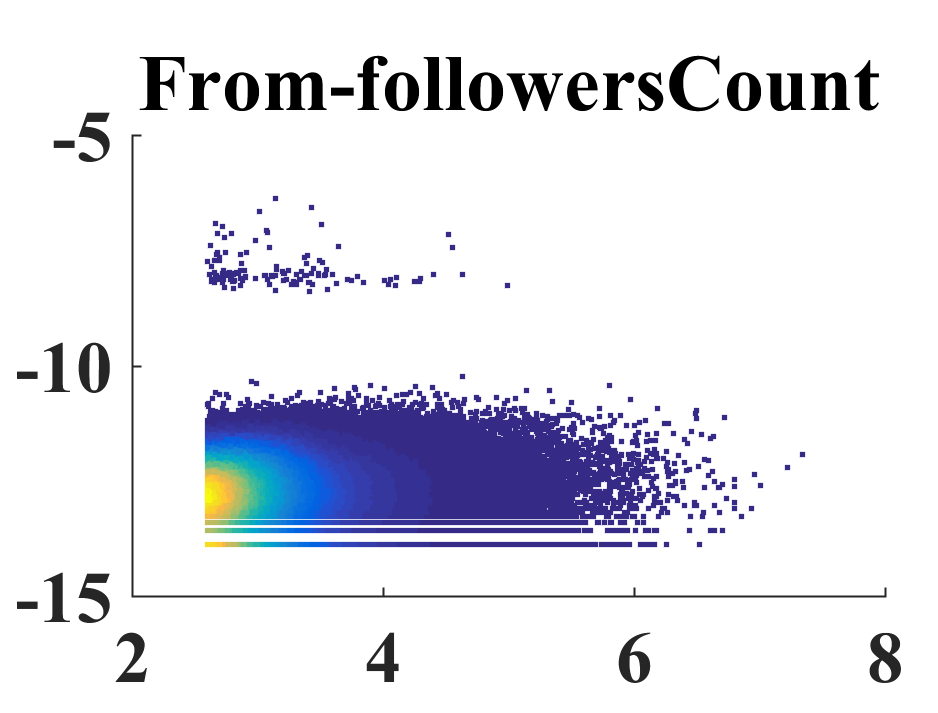
\includegraphics[width=40mm]{images/DensityPlots_IranDeal/dscatterPlot_From-followersCount.eps}} \quad
\subfloat[Fig:][]{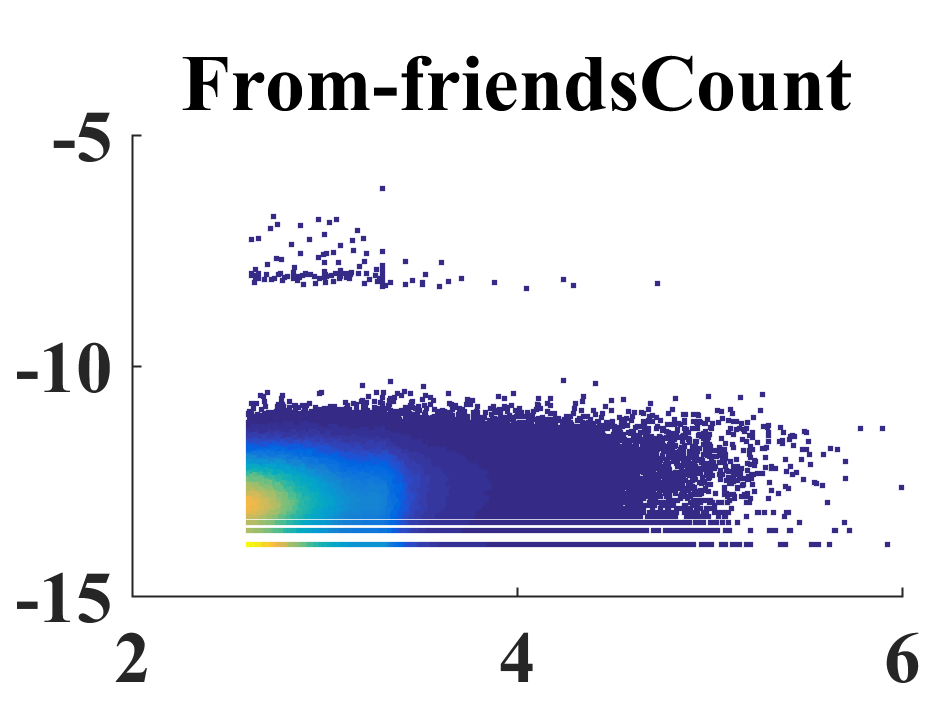
\includegraphics[width=40mm]{images/DensityPlots_IranDeal/dscatterPlot_From-friendsCount.eps}} \quad
\subfloat[Fig:][]{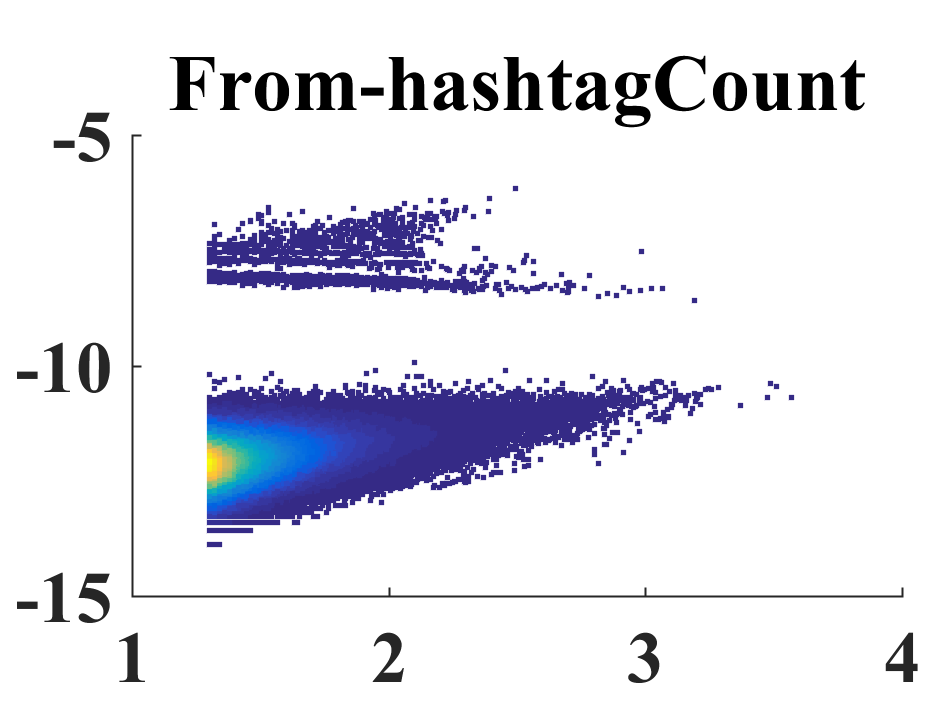
\includegraphics[width=40mm]{images/DensityPlots_IranDeal/dscatterPlot_From-hashtagCount.eps}} \\
\end{tabular}
%\vspace{-2mm} commented due to AAAI Formating
\caption {Density plots for the frequency values of feature attributes (y-axis) vs. Mutual Information (x-axis).  Plots (a-d) respectively show attributes \{favoriteCount, followerCount, friendCount, hashtagCount\} for the \textit{From} feature.}
\label{fig:densityplots}
%\vspace{2mm} commented due to AAAI Formating
\end{figure*}
\ENDCOMMENT
%%%%%%%%%%%%%%%%%%%%%%%%%%%%%%%%%%%%%%%%%%%%%%%%%%%%%%%%%%%%%%%%%%

%%%%%%%%%%%%%%%%%%%%%%%%%%%%%%%%%%%%%%%%%%%%%%%%%%%%%%%%%%%%%%%%%%
\begin{table*}[t!]
\centering
{%\renewcommand{\arraystretch}{1.2} commented due to AAAI Formating
\resizebox{\textwidth}{!}{%
\begin{tabular}{|l|l|l|l|l|l|l|l|l|l|l|}
\hline
\textbf{Topics/Top10} & \textbf{NaturalDisaster} & \textbf{Epidemics} & \textbf{IranDeal} & \textbf{SocialIssues} & \textbf{LBGT} & \textbf{HumanDisaster} & \textbf{CelebrityDeath} & \textbf{Space} & \textbf{Tennis} & \textbf{Soccer} \\ \hline \hline
\textbf{From} & earthquake\_wo & changedecopine & mazandara & nsingerdebtpaid & eph4\_15 & ydumozyf & nmandelaquotes & daily\_astrodata & tracktennisnews & losangelessrh \\ \hline
\textbf{From} & earthalerts & drdaveanddee & hhadi119 & debtadvisoruk & mgdauber & syriatweeten & boiknox & freesolarleads & tennis\_result & shoetale \\ \hline
\textbf{From} & seelites & joinmentornetwk & 140iran & debt\_protect & stevendickinson & tintin1957 & jacanews & houston\_\_jobs & i\_roger\_federer & sport\_\_agent \\ \hline
\textbf{From} & globalfloodnews & followebola & setarehgan & negativeequityf & lileensvf1 & sirajsol & ewnreporter & star\_wars\_gifts & tennislessonnow & books\_you\_want \\ \hline
\textbf{From} & gcmcdrought & localnursejobs & akhgarshabaneh & dolphin\_ls & truckerbooman & rt3syria & paulretweet & lenautilus & kamranisbest & makeupbella \\ \hline \hline
\textbf{Hashtag} & earthquake & health & iran & ferguson & tcot & syria & rip & science & wimbledon & lfc \\ \hline
\textbf{Hashtag} & haiyan & uniteblue & irantalks & mikebrown & p2 & gaza & riprobinwilliams & starwars & usopen & worldcup \\ \hline
\textbf{Hashtag} & storm & ebola & rouhani & ericgarner & pjnet & isis & ripcorymonteith & houston & tennis & arsenal \\ \hline
\textbf{Hashtag} & tornado & healthcare & iranian & blacklivesmatter & uniteblue & israel & mandela & sun & nadal & worldcup2014 \\ \hline
\textbf{Hashtag} & prayforthephilippines & depression & no2rouhani & fergusondecision & teaparty & mh370 & nelsonmandela & sxsw & wimbledon2014 & halamadrid \\ \hline \hline
\textbf{Location} & philippines & usa & tehran & st.louis & usa & malaysia & southafrica & germany & london & liverpool \\ \hline
\textbf{Location} & ca & ncusa & u.s.a & mo & bordentown & palestine & johannesburg & roodepoort & uk & manchester \\ \hline
\textbf{Location} & india & garlandtx & nederland & usa & newjersey & syria & capetown & houston & india & london \\ \hline
\textbf{Location} & newdelhi & oh-sandiego & iran & dc & sweethomealabama! & israel & pretoria & austin & pakistan & nigeria \\ \hline
\textbf{Location} & newzealand & washington & globalcitizen & washington & aurora & london & durban & tx & islamabad & india \\ \hline \hline
\textbf{Mention} & oxfamgb & foxtramedia & 4freedominiran & deray & jjauthor & ifalasteen & nelsonmandela & bizarro\_chile & wimbledon & lfc \\ \hline
\textbf{Mention} & weatherchannel & obi\_obadike & iran\_policy & natedrug & 2anow & revolutionsyria & realpaulwalker & nasa & usopen & arsenal \\ \hline
\textbf{Mention} & redcross & who & hassanrouhani & antoniofrench & govchristie & drbasselabuward & robinwilliams & j\_ksen & andy\_murray & realmadriden \\ \hline
\textbf{Mention} & twcbreaking & obadike1 & un & bipartisanism & a5h0ka & mogaza & rememberrobin & jaredleto & serenawilliams & ussoccer \\ \hline
\textbf{Mention} & abc7 & c25kfree & statedept & theanonmessage & barackobama & palestinianism & tweetlikegiris & 30secondstomars & espntennis & mcfc \\ \hline \hline
\textbf{Term} & philippines & health & iran & police & obama & israel & robin & cnblue & murray & madrid \\ \hline
\textbf{Term} & donate & ebola & regime & protesters & gun & gaza & williams & movistar & tennis & goal \\ \hline
\textbf{Term} & typhoon & acrx & nuclear & officer & rights & israeli & nelson & enero & federer & cup \\ \hline
\textbf{Term} & affected & medical & iranian & protest & america & killed & mandela & ΍imperdible & djokovic & manchester \\ \hline
\textbf{Term} & relief & virus & resistance & cops & gop & children & cory & greet & nadal & match \\ \hline
\end{tabular}
}}
\caption{The top 5 features for each feature type and topic based on Mutual Information.}
\label{table:top10MItopicsLocations}
\end{table*}
%%%%%%%%%%%%%%%%%%%%%%%%%%%%%%%%%%%%%%%%%%%%%%%%%%%%%%%%%%%%%%%%%%

%\textbf{What we have to work with: topics, features, feature attributes}
We now analyze the informativeness of our defined
features in Sec~\ref{sec:datasetStatistics} and the effect of their
attributes on learning targeted topical classifiers. 
%To this end,
%our goal in this section is to answer the following questions:
%\begin{itemize}
%\item What are the best features for learning classifiers and do they differ by topic?
%\item For each feature type, do any attributes correlate with importance?
%\end{itemize}
%To answer these questions, 
We use Mutual Information (MI)~\cite{manning_ir} as our primary
metric for feature evaluation,   
%Mutual Information is a general method
%for measuring the amount of information one random variable contains
%about another random variable and is used to select
%predictive features in machine learning.  To calculate the amount of
%information that each feature
%$j \in \{ \textit{From} \cup \textit{Hashtag} \cup \textit{Mention} \cup \textit{Term} \cup \textit{Location} \}$
%provides w.r.t.\ each topic label $t \in \{NaturalDisaster, Epidemics,...\}$,
%Mutual Information is formally defined as 
%\begin{align*}
%I(j, t) & = \!\!\! \sum_{t \in \{ \mathrm{0}, \mathrm{1} \}} \sum_{j \in \{ \mathrm{0}, %\mathrm{1}\}}p(j,t)\log \left ( \frac{p(j,t)}{p(j)p(t)} \right ) , 
% \label{eq:eq1}
%\end{align*}
%with marginal probabilities of topic $p(t)$ and feature $p(j)$ occurrence and joint probability $p(t,j)$ computed over the sample space of all tweets, 
where higher values for this metric indicate more informative features for the given topic.

%In order to answer the first question regarding the best features
%for learning topical classifiers, 
We provide the mean Mutual Information
values for each feature across different topics in Fig.~\ref{fig:avgMI}.
The last column in Fig.~\ref{fig:avgMI} shows the
average of the mean Mutual Information for each feature type.  We observe
the following:
\begin{itemize}%[noitemsep] %nolistsep
\item The \textit{Term} and \textit{Location} features are the most informative features on average (despite class labels being \emph{Hashtags}).% and in general, the more features you have, the better the chance that one is useful.
%\item There are a few topics such as \textit{IranDeal} and \textit{tennis}, that are less sensitive to the selection of a specific set of features and are in the list of top $4$ MAP scores of \textit{Logistic Regression}.%providing evidence on the power of learning social sensors for these cases.
\item The \textit{Location} feature provides the highest MI regarding the topics of \textit{HumanDisaster}, \textit{LBGT}, and \textit{Soccer} indicating that the content in these topics is heavily localized.
\item Looking at the overall average values, the order of informativeness of feature types appears to be the following: \textit{Term}, \textit{Location}, \textit{Hashtag}, \textit{Mention}, \textit{From}.
\end{itemize}
%To further analyze the relationship between the informativeness of feature types and topics,
%we refer to the box plots of Fig.~\ref{fig:avgMIBP}.  Here we see the quartiles and outliers of
%the distribution rather than just the average of the MI values in order to ensure the mean MI
%values were not misleading our interpretations.  Overall, the story is the same: term
%and location features dominate in terms of MI followed by the other less informative
%features.  Furthermore, two observations are apparent: (1) terms have more outliers indicating that
%\emph{the most useful individual features may be terms}, and (2) the topic has little impact on which feature
%is most important indicating \emph{stability of feature type informativeness over topics}.

As anecdotal evidence to support these conclusions and provide additional insights regarding
the informativeness of each feature type, we refer to
Table~\ref{table:top10MItopicsLocations}, which displays the top five feature instances
for each feature type and topic.  Among many remarkable insights in this table, one key aspect  
we note is that the \emph{terms appear to be the most generic} (and hence most generalizable) features,
providing strong intuition as to why these features are informative over the two year time
span of our data.  The top \emph{locations are also highly relevant to most topics} indicating
the overall importance of these tweet features for identifying topical tweets.


% Need more insight than this! -SPS
%
%It can be observed that the different locations, hashtags, or terms
%shown as the top features based on Mutual Information are actually in
%relation with the specific topic.

\COMMENT
In order to answer the second question on whether any attributes
correlate with importance for each feature, we provide two types of
analysis. The first analysis shown in Fig.~\ref{fig:violinplots}
analyzes the distributions of Mutual Information values for features
when binned by the magnitude of various attributes of those
features, outlined as follows:
\begin{itemize}
\item \textbf{From} vs. 
\begin{itemize}
\item \textit{Favorite count:} \# of tweets user has favorited.
\item \textit{Followers count:} \# of users who follow user.
\item \textit{Friends count:} \# of users followed by user.
\item \textit{Hashtag count:} \# of hashtags used by user.
\item \textit{Tweet count:} \# of tweets from user.
 \end{itemize}
\end{itemize}
\begin{itemize}
\item \textbf{Hashtag} vs.
\begin{itemize}
\item \textit{Tweet count:} \# of tweets using hashtag.
\item \textit{User count:} \# of users using hashtag.
\end{itemize}
\end{itemize}
\begin{itemize}
\item \textbf{Location} vs. \textit{User count:} \# of users using location.
\item \textbf{Mention} vs. \textit{Tweet count:} \# of tweets using mention.
\item \textbf{Term} vs. \textit{Tweet count:} \# of tweets using term.
\end{itemize}
As we can see in the Violin plots of Fig.~\ref{fig:violinplots}, the
general pattern is that the greater the number of tweets, users, or
hashtag count a feature has, the more informative the feature is in general.
This pattern also exists to some extent on the attributes
of the \textit{From} feature, although the pattern is less visible in
general and not clear (or very weak) for the follower or friend count.
In general, the informativeness of a user appears to have little correlation
with their follower or friend count.

Fig.~\ref{fig:densityplots} provides a further analysis by showing
density plots of favorite count, follower count, friends count, and
hashtag count attributes of the \textit{From} feature.  Here we see an
interesting phenomenon that was not clear in the Violin plots: there
is a very clear bimodality of the density.  On further investigation
it turns out that the top mode feature occurs in at least one topical
tweet whereas the bottom mode occurs in no topical tweets.  While the
bottom mode features may serve as good indicators of non-topicality,
the top mode are inherently more indicative of topicality, which
justifies feature selection by mutual information.
\ENDCOMMENT
